\chapter{Introduction}
Recent studies from Pew Research Centre have shown that a substantial amount of population from major African countries will be migrating in the next five years to Western and European countries for a better lifestyle which they are lacking in their country. Poverty is one of the most important factors to be looked at while deriving the economic status of a particular region\cite{jean2016combining}. Having a well formed data and record of poverty of a region can help the government and other organizations make informed decisions and implement certain policies that can work towards eradicating it. This can be done by collecting various kinds of data on the well being of the people of a particular place. Conducting surveys can be a method for data collection, but it is not practical in most of the regions as the accessibility is low, they tend to be expensive and time consuming. With the advancements of remote sensing, machine learning and image processing efficient predictive algorithms can be developed to analyze the socioeconomic factor of different regions and take precautionary actions before things get worse.

Battling the deficiency of reliable poverty data in the developing countries have been a challenge, hence there is a need for a cheap and scalable method of collecting such data to facilitate the economic progress in these areas. Some of the ways which can help in determining economic activity in vast geographic regions are:
\begin{itemize}
    

\item Night time luminous intensity using remote sensing.
\item Distribution of household structures and their parameters.
\item Automobile activity.
\end{itemize}

\section{Overview}
This chapter provides the information related to the work which includes background, the purpose, goal, methodology followed and the stakeholders of the project.

\section{Background}
\label{sec:background}


The economic status or livelihood is quite difficult to predict due to the scarcity of reliable data sets from various developing countries~\cite{jean2016combining}. Also topics like these are very crucial for both research and political purposes. In the recent years, though this kind of data has increased in quality and quantity due to widespread surveys being conducted and the emergence of new technologies which can capture the data easily. Even if this data gap exists, the \ac{DHS} program collects accurate data on health and population of developing countries. It provides us with valuable wealth distribution and household information in that region. It covers more than ninety countries worldwide now~\cite{mullainathan2017machine}.
 
The difficulties in collecting this data is that it requires a lot of human effort and lots of cost associated with it. Therefore, another reliable data source was needed. Hence a recent approach of using the satellite images of night light luminous intensity to predict the economic activity in the selected regions~\cite{pokhriyal2017combining}. These images taken from  \ac{NOAA} gives the stack of satellite images during night time captured during 8:30 PM to 10:30 PM. This visualization shows only the lights generated from electricity~\cite{jin2017method}.

Nightlight images do not expose geographical features, which can be found only on the Daytime captured satellite visuals giving a clear view of infrastructure, buildings, roads, farmland, etc. in a particular area. The Daytime satellite images are taken from Google Static Maps. The Google \ac{API} Key is required to download these images. They have a luminosity range of $0$ to $63$, where $0$ is no luminosity at all and $63$ being the most luminous and is spread across $1 km^2$ with a zoom level of $16$. As these are satellite images, only a little zooming will enlarge it to a great extent. Thus, this is the optimal value to be considered~\cite{chen2006remote}.


\begin{figure}[h!]
\centering
\begin{tikzpicture}[spy using outlines={circle,yellow,magnification=2,size=2.5cm, connect spies}]
\node{\pgfimage[width=0.9\columnwidth]{setup/img/nightlight}};
\spy on (0.6,-0.2) in node [left] at (4,-1.5);
\end{tikzpicture}
\vspace{-0.2cm}
\caption{\newline Sample of night-time luminous intensity satellite image~\cite{kyba2017artificially}. Magnification from Nigeria to Mozambique.
This composite image, shows a global view of Earth at night, compiled from over 400 satellite images. The nighttime light data (2017) was recorded by the Defense Meteorological Satellite Program (DMSP) in the National Geophysical Data Center (NGDC), a part of NOAA. Image Credit: NASA/NOAA.}
\label{fig:sample_of_night_light}
\end{figure}


\section{Problem}
Using just the survey data to predict poverty is time consuming and expensive. Due to lack of transportation and resources, performing such surveys and reaching each and every household is not feasible. With such an anonymous data how can one perform the analysis to determine the poverty of a region?

%Use acronyms:
%The \ac{NOAA} is very nice. It is a \ac{NOAA}

\section{Purpose}
 The project illustrates a methodology to determine the poverty of selected regions using satellite imagery thus helping the nations to take required measures to improve the economic situation. The agricultural improvements can be done in different regions of the nations. Loans can be provided to the needy depending on the situations from the Fintech groups. This work helps the \ac{NGO}s and Governments to grant resources to help these under developed nations by analysing the poverty data.


\section{Goal}
The goal of this project is to build an efficient model which can predict the socioeconomic status of different countries using remote sensing, survey data and google maps.
% The results show the performance analysis of the the models built, based on the correlation between the actual wealth as observed in the survey data and the wealth index predicted by the model. The predicted wealth is mapped on a heat map for visualizing the wealth distribution of the particular regions.

\section{Benefits, Ethics and Sustainability}
If proper measures are taken, both the government and the people get benefited from this work. The per capita income increases and the livelihood of the people becomes better.


\section{Methodology}

This research focuses on the countries in the African continent.
The proposed model is depicted by the flow diagram shown in Fig.~\ref{fig:proposed_model}. It subsumes three stages of core operations: data collection and pre-processing, transfer learning, and training and prediction. The following subsections elaborate each of the stages.



\begin{figure*}[h!]
\centering
  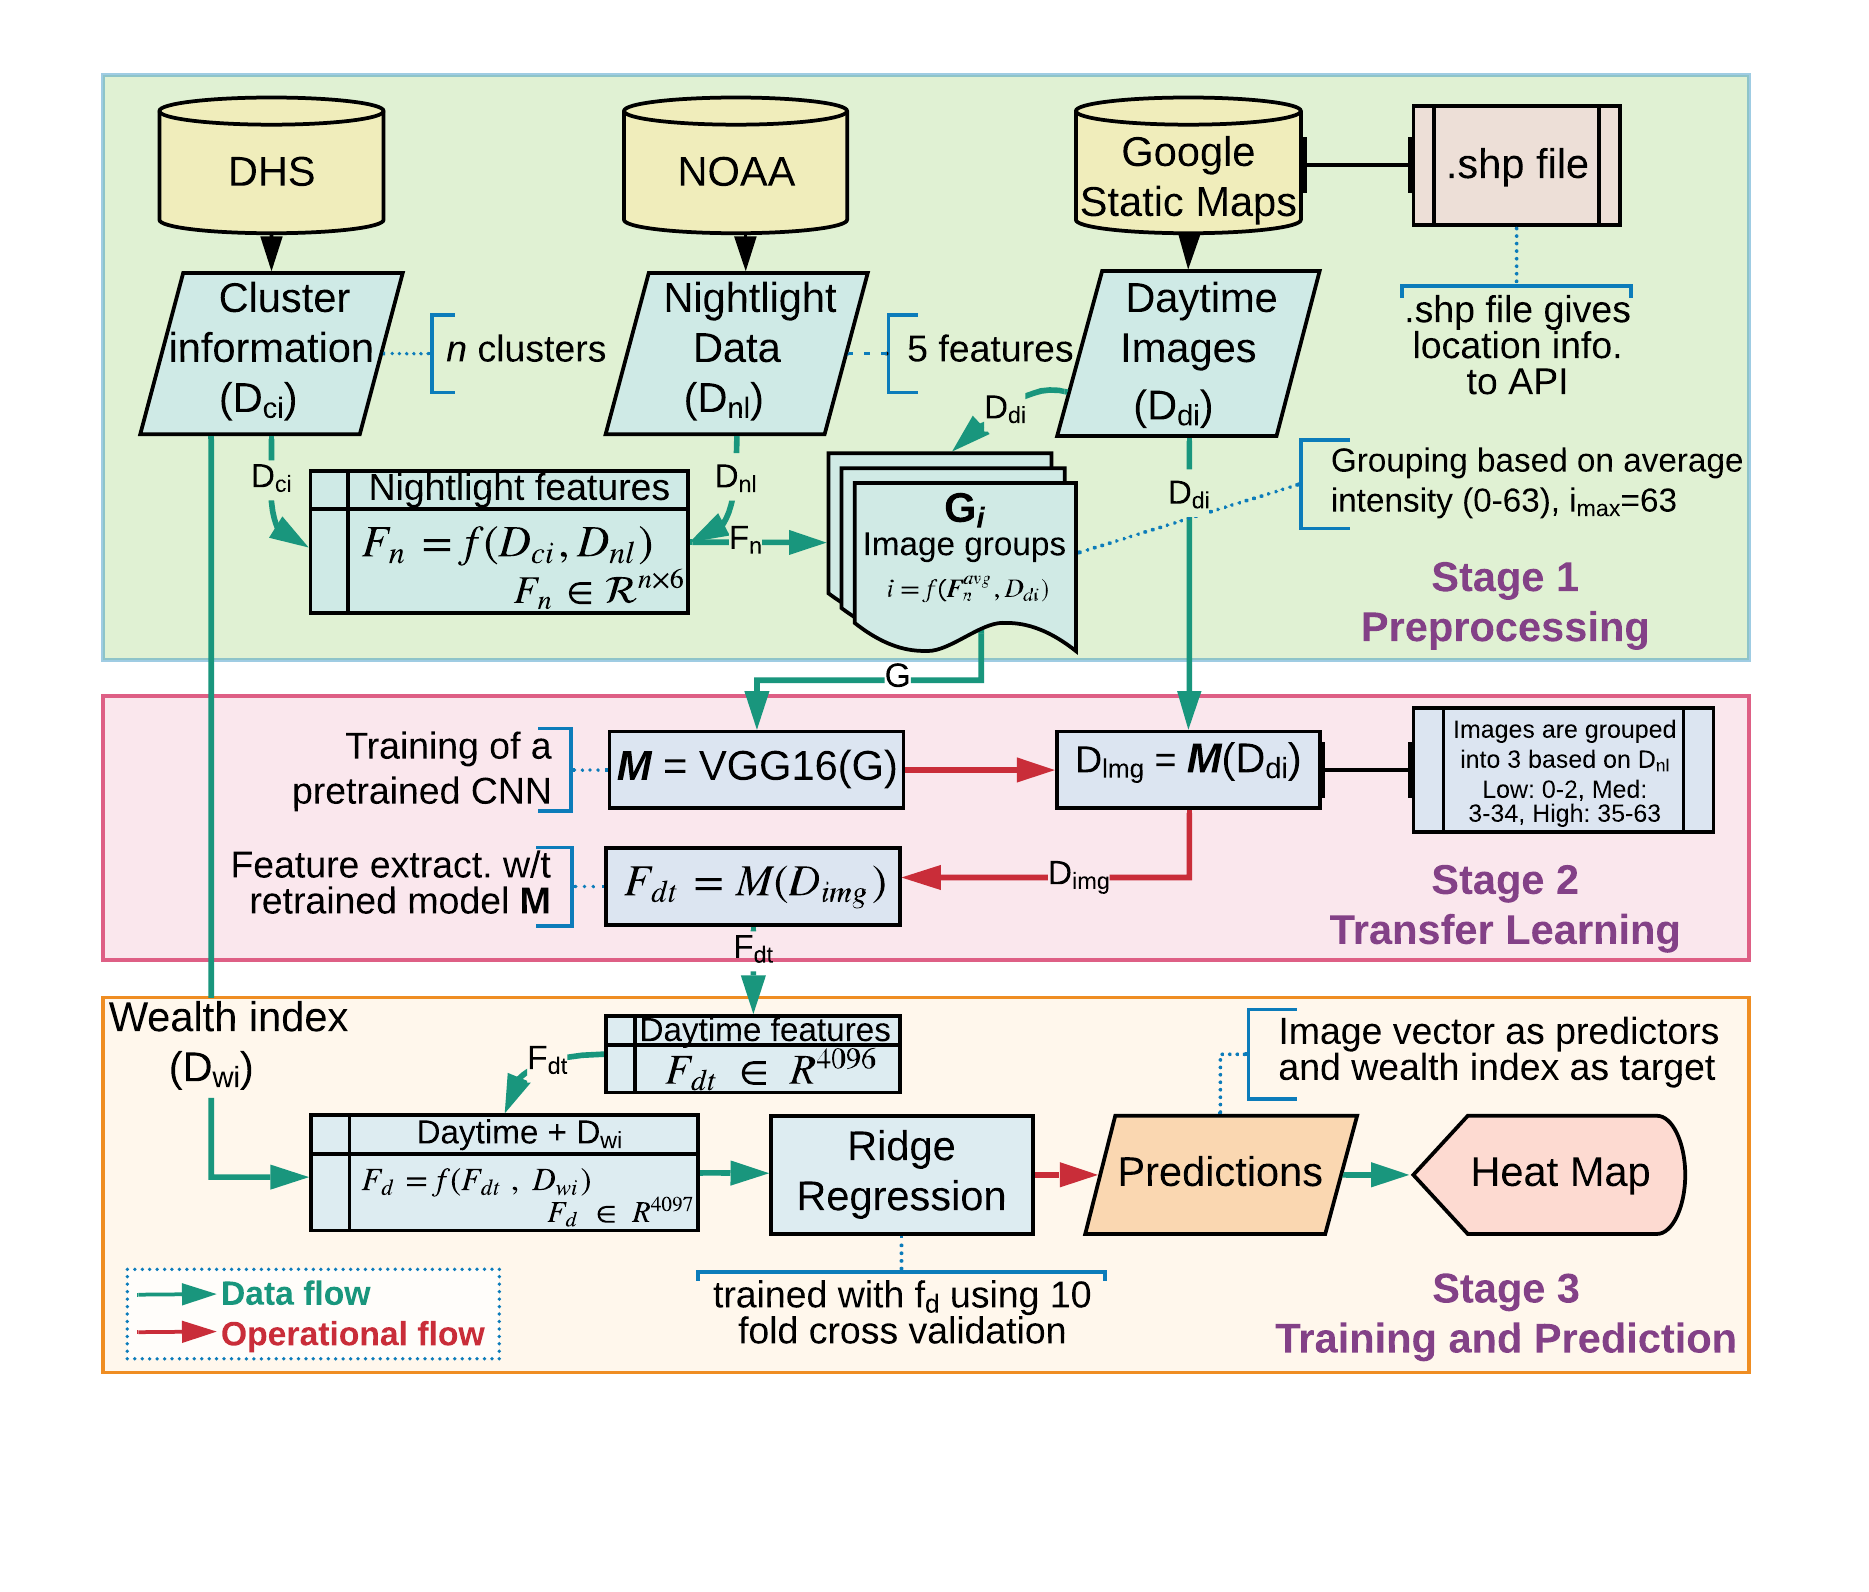
\includegraphics[width=0.99\textwidth]{setup/img/projectfinalflowchart.png}
  \caption{The operational flow of the proposed solution for socioeconomic prediction.}
  \label{fig:proposed_model}
  \centering
\end{figure*}

  


\subsection{Stage 1: Data collection and Preprocessing}
This research focuses on the countries in the African continent, such as, Rwanda, Madagascar, Mozambique, and Nigeria. 
The reason behind choosing these countries is that the majority of the population are still without electricity and the availability of electricity has always been a good representation of the economic status of a region. For the aforesaid regions the following data are collected: NOAA, DHS, and Google Static Maps.

The DHS consists of household records, which includes location information and socioeconomic variables of a particular cluster. We retrieve the household cluster information (latitude, longitude) and the geographic data (shape file) of the particular country selected from DHS. The shape file defines the region boundaries (nation, province, districts etc.). Secondly, NOAA consisting of a high definition raster file, which holds all the nightlight information from which the nighttime satellite images are extracted. The features in the nightlight data are Min, Max, Median, Mean, Standard deviation. Thirdly, Google Static Maps, from which the Daytime satellite images are downloaded using the sector boundary shape file as an input for locations to the API. Basic image features are extracted from the daylight images (simple image metrics). These features are merged with \ac{DHS}, and the regression score is considered in order to test whether they can be used to predict the wealth index. We extract the nightlight features, which contains concatenated features of cluster information and nightlight data with the help of \ac{GDAL} (Geospatial Data Abstraction Library) which is used to read and write the raster and geospatial data formats. We group the satellite images based on average nightlight intensities ($0$-$63$), where $0$ being the lowest intensity and $63$ being the highest intensity.


\subsection{Stage 2: Transfer Learning}

There are only several hundred consumption data points or properties in each country to be used as labelled training examples, it cannot be precisely trained on a broad Convolutional Neural Network (CNN)-based model to estimate such outcomes from satellite images. 
% We do not have enough data. 
To counter the data shortage, we adopt the transfer learning method. Transfer learning enables one to use the knowledge gained from a proxy task into performing a related actual task~\cite{8122666}, in our case the proxy task being the classification based on the abundantly available nightlight data and the actual task being the feature extraction from the daytime images.

To do this, first a \ac{CNN} is trained on a task of high intensity night light estimation. Here, we fine-tune a previously trained VGG 16 on ImageNet to estimate night-time light intensity at different locations, according to the corresponding daytime satellite images. 
% The CNN is used for a classification task where the daylight images are classified into three classes based on night light intensity low, medium, and high.
Due to the global availability of night light data at a resolution of $1 km$, the inputs are $400 \times 400$ pixel daytime satellite images from Google Static Maps at zoom level $16$, which approximately corresponds to $1~km^2$. The day time images are from the year 2019 and the high resolution nightlight image used is from 2017. After the \ac{CNN} model has been trained to classify the images based on the intensity of nightlight into three classes: low (0-2), medium (3-34), and high (35-63), we use this model as a daytime satellite image feature extractor from every cluster that consists of $m$ number of layers by discarding the last layer of the \ac{CNN} model which is the nightlight classification layer. Thus, a cluster is to have a feature vector $\mathbf{F}^c_{dt} \in \mathbb{R}^{m\times 4096}$. This will be further processed by a dimensionality reduction operator $\myfunc{g}$, like:
\begin{equation}
    \mathbf{F}^c_{dt} = \myfunc{g}(\mathbf{F}^c_{dt}), 
    \label{eqn:avg_op}
\end{equation}
where a country may have $C$ number of cluster with a cluster index, $c={1,...,C}$ and $\myfunc{g}$ is a row-wise average operation. Consequentially, a cluster $c$ will have a daytime satellite image feature representation w.r.t night-time luminous values, as $\mathbf{F}^c_{dt} \in \mathbb{R}^{4096}$.

\subsection{Stage 3: Training and Prediction}

This is the stage where the training and predictions take place. Wealth index to corresponding daytime features extracted using the \ac{CNN} re-trained on Nightlight features and is predicted using a ridge regression model. We have conducted trials in which our training labels have been randomly adjusted so that every training example has a randomly paired image vector and wealth label. Each trial tested on a $10$-fold or a $5$-fold cross-validation frame regression model, again selecting regularisation variables in a nested cross-validation mode and after that the image feature dimension is reduced to $100$ using \ac{PCA}. We are plotting the \( R^2\) distribution based on the nightlight intensities and cluster wealth. Using the extracted features and the predicted wealth index, we plot the heat maps. The heat maps show the wealth distribution concluding the Socioeconomic status of the country.





\section{Stakeholders}
Sree Teja Varma Buddaraju, Ananya Bardhan, Ramya Sri Boddu, Simranjit Kaur, Thangarajah~Akilan,~\IEEEmembership{Member,~IEEE}

%\section{Delimitations}
%Explain the delimitations. These are all the things that could affect the study if they were examined and included in the degree project. 
%Use references!

\section{Outline}
The rest of the report is structured as follows:  
\begin{itemize}
    \item Chapter 2 describes the background which is the related work of this work.
    \item Chapter 3 describes the methodologies and methods. It includes information about Ridge Regression, Evaluation matrix and Data sets used for this project.
    \item Chapter 4 describes the work done in this project. It discusses about the impact of data normalization, sanity tests performed, Domain-Specific and Cross-Domain analysis and comparisons between Ridge, Linear and Lasso Regressions.
    \item Chapter 5 describes the results obtained.
    \item Chapter 6 describes the conclusions and discuses the future work.
\end{itemize}
  
